\section{动量}

\subsection{动量守恒定律}

\begin{proset}
    如图，质量为\(m\)的物块从离地面高度为\(h\)处由静止释放，同时一颗质量为\(m\)的子弹在与物块等高处沿水平方向射入物块并留在物块中，物块落地点离\(P\)点的水平距离也为\(h\)，不计物块大小，子弹打物块的时间可以忽略不计，重力加速度为\(g\)。
    \begin{enumerate}[(1)]
        \item 子弹打物块过程中子弹和物块系统损失的动能为多少？
        \item 仅改变子弹水平射出的高度，先释放物块再射出子弹，子弹恰好沿水平方向击中物块并留在物块中，结果物块落地点离\(P\)点的水平距离为\(\frac{1}{2}h\)，则调整后子弹射出的高度为多少？
    \end{enumerate}
    \begin{tikzpicture}[font=\scriptsize]
        \draw[dashed,cyan] (0,3)coordinate(p) parabola bend(0,3) (3,0) (0,3)--(0,0);
        \draw[fill=orange!40] ($(p)+(-.1,-.1)$) rectangle ++(.2,.2)node[above left] {\(P\)};
        \draw[fill=brown!60] (-.3,3)--++(-.2,.05)--++(0,-.1)--cycle;
        \foreach \x in{-.6,-.4,...,3.4}
            \draw[gray] (\x,-.2)--++(.2,.2);
        \draw[thick] (-.6,0)--(3.4,0);
    \end{tikzpicture}
\end{proset}
\begin{answer}
    （1）\(\Delta E_k = \frac{1}{2}mgh\)（2）\(\frac{1 + \sqrt{13}}{8}h\)\qquad 注意第（2）问中水平竖直两个方向上动量守恒
\end{answer}

\subsection{类碰撞模型}

\begin{proset}
    （多选）
    如图所示，光滑的水平面上有\(A\)、\(B\)、\(C\)三个物块，\(A\)、\(C\)质量均为\(m\)，\(B\)质量为\(3m\)，\(A\)、\(B\)用一根弹簧栓接并处于静止状态。某时刻，物块\(C\)以速度\(v_0\)向左运动，并与\(A\)发生碰撞，碰后\(A\)、\(C\)共速但不粘连，整个过程中，下列说法正确的是\paren[]

    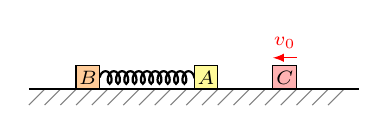
\begin{tikzpicture}[font=\scriptsize]
        \draw[thick,decoration={aspect=.6,segment length=3,amplitude=.8mm,coil},decorate] (.3,.15)--(1.6,.15);
        \draw[fill=orange!40] (0,0) rectangle(.3,.3)node[midway,black]{\(B\)};
        \draw[fill=yellow!40] (1.5,0) rectangle(1.8,.3)node[midway,black]{\(A\)};
        \draw[fill=red!30] (2.5,0) rectangle(2.8,.3)node[midway,black]{\(C\)};
        \draw[red,-latex] (2.8,.4)--node[above]{\(v_0\)}(2.5,.4);
        \foreach \x in{-.6,-.4,...,3.4}
            \draw[gray] (\x,-.2)--++(.2,.2);
        \draw[thick] (-.6,0)--(3.6,0);
    \end{tikzpicture}
    \begin{choices}
        \item 弹簧的最大弹性势能为\(\frac{3mv_0^2}{20}\)
        \item 弹簧第一次恢复原长时，物块\(B\)的速度大小为\(\frac{2v_0}{5}\)
        \item 物块\(C\)的最终速度大小为\(\frac{v_0}{5}\)
        \item 弹簧最长时的弹性势能为\(\frac{3}{32}mv_0^2\)
    \end{choices}
\end{proset}
\begin{answer}
    ABD\quad 提示：
\end{answer}

\subsection{非对心碰撞}

\begin{proset}
    台球是一项深受青少年喜爱的体育运动。如图所示，水平台面上的甲球球心和中袋中心连线与桌边间夹角\(\theta =\) \,\qty{60}{\degree}，运动员球杆将白球乙沿与桌面平行的方向以速度\(v_0\)出击，乙与甲碰撞后甲落入中袋。已知两球质量、半径均相等，两球碰撞为弹性碰撞，不计两球所受阻力，不考虑球的自旋影响。关于甲、乙两球的运动，下列说法正确的是\paren[]

    \begin{tikzpicture}
        \draw[dashed] (0,0)node[above,font=\tiny]{\kaishu 中袋}--(-60:{2*sqrt(3)/3})coordinate(a)--++(1,0)coordinate(b);
        \draw[fill=white] (-2,-.2) arc(-90:0:.2) (-1.8,-2) arc(0:90:.2) (1.8,-2) arc(-180:-270:.2) (2,-.2) arc(-90:-180:.2) (.2,-2)arc(0:180:.2) (.2,0)arc(0:-180:.2)  ($(a)+(120:.2)$)node[left,font=\tiny]{\kaishu 甲} circle(.1) (b) circle(.1)node[below,font=\tiny]{\kaishu 乙};
        \draw[fill=white,dashed] (a) circle(.1);
        \draw (-2,0) rectangle(2,-2);
        \draw[red,->] ($(b)+(-.1,0)$)--++(-.4,0)node[above,font=\scriptsize]{\(v_0\)};
    \end{tikzpicture}
    \begin{choices}
        \item 碰撞后乙球速度方向不变
        \item 碰撞后两球速度方向垂直
        \item 碰撞后甲球速度大小为\(\frac{\sqrt{3}}{2}v_0 \)
        \item 碰撞后乙球速度大小为\(\frac{v_0}{2}\)
    \end{choices}
\end{proset}
\begin{answer}
    B\quad 提示：
\end{answer}

\subsection{相对速度}

\begin{proset}
    （多选）
    如图所示，半径为\(R\)的光滑半球放在光滑水平面上，将一小滑块（可视为质点）轻放在半球的顶端，小滑块和半球均处于静止状态。在外界微小扰动下，小滑块从静止开始沿球面自由滑下，当小滑块与球心连线与竖直方向夹角\(\theta =\) \,\qty{37}{\degree}时，小滑块离开球面。重力加速度为\(g\)，\(\sin\) \,\qty{37}{\degree}\( = 0.6\)，\(\cos\) \,\qty{37}{\degree}\( = 0.8\)，下列说法正确的是\paren[]

    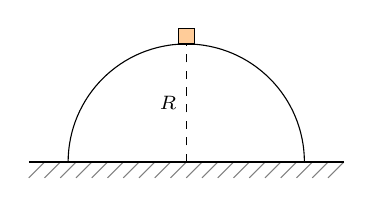
\begin{tikzpicture}
        \draw (1.5,0) arc(0:180:1.5);
        \foreach \x in{-2,-1.8,...,1.8}
            \draw[gray] (\x,-.2)--++(.2,.2);
        \draw[thick] (-2,0)--(2,0);
        \draw[dashed] (0,0)--node[left,font=\scriptsize]{\(R\)}(0,1.5);
        \draw[fill=orange!40] (-.1,1.5) rectangle(.1,1.7);
    \end{tikzpicture}
    \begin{choices}
        \item 小滑块在球面上滑动过程中，小滑块与半球组成的系统动量守恒
        \item 小滑块在球面上滑动过程中，小滑块与半球组成的系统机械能守恒
        \item 小滑块离开半球时，半球的速度大小为\(\frac{\sqrt{5gR}}{4}\)
        \item 小滑块离开半球时，半球移动的距离为\(\frac{17}{32}R\)
    \end{choices}
\end{proset}
\begin{answer}
    BC\quad 提示：

    \begin{tikzpicture}[font=\scriptsize,>=latex]
        \draw[gray] (2,0) arc(0:180:2);
        \foreach \x in{-2.4,-2.2,...,2.2}
            \draw[gray] (\x,-.2)--++(.2,.2);
        \draw[thick] (-2.4,0)--(2.4,0);
        \draw[dashed] (0,0)--(53:2)coordinate(a);
        \draw[->,red] (a)--++(-37:1.6)coordinate(u)node[right]{\(u\)};
        \draw[->,blue] (a)--++(0:-1)coordinate(c)node[left]{\(v_2\)};
        \draw[->,cyan] (a)--++($(-37:1.6)+(-1,0)$)coordinate(b)node[below]{\(v_1\)};
        \draw[dashed] (c)--(b)--(u)|-(a) (b)|-(a-|2,1.6);
        \draw[->,cyan] (a)--++(.3,0)node[above]{\(v_{1x}\)};
        \fill (a) circle(.03) (0,0) circle(.03);
    \end{tikzpicture}

    小滑块的速度\(v_1\)、半球的速度\(v_2\)及滑块相对半球的速度\(u\)的关系如图所示，小滑块质量\(m\)、半球质量\(M\)系统水平方向动量守恒：\( Mv_2 =mv_{1x} = m(u\cos\theta - v_2)\)

    由能量守恒可得：\(mgR(1 -\cos\theta) = \frac{1}{2}Mv_2^2 + \frac{1}{2}mv_1^2 = \frac{1}{2}Mv_2^2 + \frac{1}{2}m[(u\sin\theta)^2 +(u\cos\theta - v_2)^2]\)

    小滑块相对半球做圆周运动，\(\theta =\) \,\qty{37}{\degree}时恰好脱离，可得：\(mg\cos\theta = m \frac{u^2}{R}\)

    解得：\(M:m = 7:25\)\quad \(u = \frac{2 \sqrt{5gR}}{5}\)\quad \(v_2 = \frac{\sqrt{5gR}}{4}\)\quad \(x_2 = \frac{25}{7 + 25}\cdot R\sin\theta = \frac{15}{32}R\)
\end{answer}

\subsection{连续碰撞}

\begin{proset}
    如图所示，一足够长的固定斜面倾角为\(\theta =\) \,\qty{30}{\degree}，质量为\(m_1 =\) \,\qty{1}{kg}的物块\(A\)与静止在斜面上的质量为\(m_2 =\) \,\qty{0.5}{kg}的物块\(B\)发生第一次碰撞前瞬间，物块\(A\)的速度为\(v_0 = \frac{4}{3}\) \,\qty{}{m/s}，\(A\)和\(B\)的碰撞均为弹性碰撞且碰撞时间极短，\(A\)、\(B\)与斜面之间的动摩擦因数分别为\(\mu_1 = \frac{\sqrt{3}}{3}\)、\(\mu_2 = \frac{\sqrt{3}}{2} \)，\(A\)、\(B\)均可视为质点，重力加速度\(g\)取\,\qty{10}{m/s^2}，不计空气阻力。求：
    \begin{enumerate}[(1)]
        \item 第一次碰撞后\(A\)和\(B\)的速度大小；
        \item \(A\)、\(B\)发生第二次碰撞前瞬间\(B\)的速度大小；
        \item \(A\)、\(B\)从第一次碰撞后到第(\(n + 1\))次碰撞前（\(n > 1\)且\(n\)非无穷大），\(B\)的位移大小。
    \end{enumerate}
    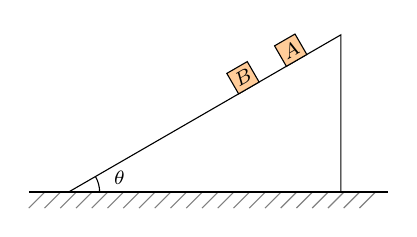
\begin{tikzpicture}[font=\scriptsize]
		\def\TheTa{30}%旋转角度
		\def\LenGth{4}%斜面长度
		\pgfmathsetmacro\CosLenGth{\LenGth*cos(\TheTa)+.4}
		\begin{scope}[rotate=\TheTa]	
			\draw (0,0)--++(\LenGth,0)--++(-120:2);
            \draw[fill=orange!40] (2.5,0) rectangle(2.8,.3)node[midway,rotate=30]{\(B\)} (3.2,0) rectangle(3.5,.3)node[midway,rotate=30]{\(A\)};
		\end{scope}
		\draw (.4,0) arc(0:\TheTa:.4);
		\node at(.65,.18){\(\theta\)};
		\foreach \x in{-.5,-.3,...,\CosLenGth}
			\draw[gray] (\x,-.2)--++(.2,.2);
		\draw[thick] (-.5,0)--({\CosLenGth+.2},0);
	\end{tikzpicture}
\end{proset}
\begin{answer}
    （1）\(v_{A1} = \frac{4}{9}\) \,\qty{}{m/s}\quad \(v_{B1} = \frac{16}{9}\) \,\qty{}{m/s}（2）0（3）\(\frac{32}{45}(1 - \frac{1}{9^n})\) \,\qty{}{m}

    注意\(\mu_1 = \frac{\sqrt{3}}{3} \)，碰撞后\(A\)做匀速直线运动，\(B\)做匀减速运动，加速度\(a = g(\mu_2\cos\theta - \sin\theta) =\) \,\qty{2.5}{m/s^2}。

    第一次碰撞后\(v_{A1} = \frac{m_1 - m_2}{m_1 + m_2}v_0 = \frac{1}{3}v_0\)\quad \(v_{B1} = \frac{2m_1v_0}{m_1 + m_2} = \frac{4}{3}v_0\)

    第二次碰撞后\(v_{A2} = \frac{1}{3}v_{A1} = \frac{1}{3^2}v_0\)\quad \(v_{B2}= \frac{4}{3}v_{A1} = \frac{4}{3^2}v_0\)

    第\(n\) 次碰撞后\(v_{An} = \frac{1}{3^n}v_0\)\quad \(v_{Bn} = \frac{4}{3^n}v_0\)

    \(B\)第\(n\)次碰撞后沿斜面下滑的位移\(x_n = \frac{v_{Bn}^2}{2a} = \frac{16^2}{5 \times 9^{n + 1}}\) \,\qty{}{m}
\end{answer}